%% LyX 2.0.3 created this file.  For more info, see http://www.lyx.org/.
%% Do not edit unless you really know what you are doing.
\documentclass{article}
\usepackage{graphicx, color}
\IfFileExists{upquote.sty}{\usepackage{upquote}}{}
\definecolor{fgcolor}{rgb}{0.267, 0.267, 0.267}
\newcommand{\hlnumber}[1]{\textcolor[rgb]{0,0,0}{#1}}%
\newcommand{\hlfunctioncall}[1]{\textcolor[rgb]{0.501960784313725,0,0.329411764705882}{\textbf{#1}}}%
\newcommand{\hlstring}[1]{\textcolor[rgb]{0.6,0.6,1}{#1}}%
\newcommand{\hlkeyword}[1]{\textcolor[rgb]{0,0,0}{\textbf{#1}}}%
\newcommand{\hlargument}[1]{\textcolor[rgb]{0.690196078431373,0.250980392156863,0.0196078431372549}{#1}}%
\newcommand{\hlcomment}[1]{\textcolor[rgb]{0.180392156862745,0.6,0.341176470588235}{#1}}%
\newcommand{\hlroxygencomment}[1]{\textcolor[rgb]{0.43921568627451,0.47843137254902,0.701960784313725}{#1}}%
\newcommand{\hlformalargs}[1]{\textcolor[rgb]{0.690196078431373,0.250980392156863,0.0196078431372549}{#1}}%
\newcommand{\hleqformalargs}[1]{\textcolor[rgb]{0.690196078431373,0.250980392156863,0.0196078431372549}{#1}}%
\newcommand{\hlassignement}[1]{\textcolor[rgb]{0,0,0}{\textbf{#1}}}%
\newcommand{\hlpackage}[1]{\textcolor[rgb]{0.588235294117647,0.709803921568627,0.145098039215686}{#1}}%
\newcommand{\hlslot}[1]{\textit{#1}}%
\newcommand{\hlsymbol}[1]{\textcolor[rgb]{0,0,0}{#1}}%
\newcommand{\hlprompt}[1]{\textcolor[rgb]{0.266666666666667,0.266666666666667,0.266666666666667}{#1}}%

\usepackage{color}%
 
\newsavebox{\hlnormalsizeboxclosebrace}%
\newsavebox{\hlnormalsizeboxopenbrace}%
\newsavebox{\hlnormalsizeboxbackslash}%
\newsavebox{\hlnormalsizeboxlessthan}%
\newsavebox{\hlnormalsizeboxgreaterthan}%
\newsavebox{\hlnormalsizeboxdollar}%
\newsavebox{\hlnormalsizeboxunderscore}%
\newsavebox{\hlnormalsizeboxand}%
\newsavebox{\hlnormalsizeboxhash}%
\newsavebox{\hlnormalsizeboxat}%
\newsavebox{\hlnormalsizeboxpercent}% 
\newsavebox{\hlnormalsizeboxhat}%
\newsavebox{\hlnormalsizeboxsinglequote}%
\newsavebox{\hlnormalsizeboxbacktick}%

\setbox\hlnormalsizeboxopenbrace=\hbox{\begin{normalsize}\verb.{.\end{normalsize}}%
\setbox\hlnormalsizeboxclosebrace=\hbox{\begin{normalsize}\verb.}.\end{normalsize}}%
\setbox\hlnormalsizeboxlessthan=\hbox{\begin{normalsize}\verb.<.\end{normalsize}}%
\setbox\hlnormalsizeboxdollar=\hbox{\begin{normalsize}\verb.$.\end{normalsize}}%
\setbox\hlnormalsizeboxunderscore=\hbox{\begin{normalsize}\verb._.\end{normalsize}}%
\setbox\hlnormalsizeboxand=\hbox{\begin{normalsize}\verb.&.\end{normalsize}}%
\setbox\hlnormalsizeboxhash=\hbox{\begin{normalsize}\verb.#.\end{normalsize}}%
\setbox\hlnormalsizeboxat=\hbox{\begin{normalsize}\verb.@.\end{normalsize}}%
\setbox\hlnormalsizeboxbackslash=\hbox{\begin{normalsize}\verb.\.\end{normalsize}}%
\setbox\hlnormalsizeboxgreaterthan=\hbox{\begin{normalsize}\verb.>.\end{normalsize}}%
\setbox\hlnormalsizeboxpercent=\hbox{\begin{normalsize}\verb.%.\end{normalsize}}%
\setbox\hlnormalsizeboxhat=\hbox{\begin{normalsize}\verb.^.\end{normalsize}}%
\setbox\hlnormalsizeboxsinglequote=\hbox{\begin{normalsize}\verb.'.\end{normalsize}}%
\setbox\hlnormalsizeboxbacktick=\hbox{\begin{normalsize}\verb.`.\end{normalsize}}%
\setbox\hlnormalsizeboxhat=\hbox{\begin{normalsize}\verb.^.\end{normalsize}}%



\newsavebox{\hltinyboxclosebrace}%
\newsavebox{\hltinyboxopenbrace}%
\newsavebox{\hltinyboxbackslash}%
\newsavebox{\hltinyboxlessthan}%
\newsavebox{\hltinyboxgreaterthan}%
\newsavebox{\hltinyboxdollar}%
\newsavebox{\hltinyboxunderscore}%
\newsavebox{\hltinyboxand}%
\newsavebox{\hltinyboxhash}%
\newsavebox{\hltinyboxat}%
\newsavebox{\hltinyboxpercent}% 
\newsavebox{\hltinyboxhat}%
\newsavebox{\hltinyboxsinglequote}%
\newsavebox{\hltinyboxbacktick}%

\setbox\hltinyboxopenbrace=\hbox{\begin{tiny}\verb.{.\end{tiny}}%
\setbox\hltinyboxclosebrace=\hbox{\begin{tiny}\verb.}.\end{tiny}}%
\setbox\hltinyboxlessthan=\hbox{\begin{tiny}\verb.<.\end{tiny}}%
\setbox\hltinyboxdollar=\hbox{\begin{tiny}\verb.$.\end{tiny}}%
\setbox\hltinyboxunderscore=\hbox{\begin{tiny}\verb._.\end{tiny}}%
\setbox\hltinyboxand=\hbox{\begin{tiny}\verb.&.\end{tiny}}%
\setbox\hltinyboxhash=\hbox{\begin{tiny}\verb.#.\end{tiny}}%
\setbox\hltinyboxat=\hbox{\begin{tiny}\verb.@.\end{tiny}}%
\setbox\hltinyboxbackslash=\hbox{\begin{tiny}\verb.\.\end{tiny}}%
\setbox\hltinyboxgreaterthan=\hbox{\begin{tiny}\verb.>.\end{tiny}}%
\setbox\hltinyboxpercent=\hbox{\begin{tiny}\verb.%.\end{tiny}}%
\setbox\hltinyboxhat=\hbox{\begin{tiny}\verb.^.\end{tiny}}%
\setbox\hltinyboxsinglequote=\hbox{\begin{tiny}\verb.'.\end{tiny}}%
\setbox\hltinyboxbacktick=\hbox{\begin{tiny}\verb.`.\end{tiny}}%
\setbox\hltinyboxhat=\hbox{\begin{tiny}\verb.^.\end{tiny}}%



\newsavebox{\hlscriptsizeboxclosebrace}%
\newsavebox{\hlscriptsizeboxopenbrace}%
\newsavebox{\hlscriptsizeboxbackslash}%
\newsavebox{\hlscriptsizeboxlessthan}%
\newsavebox{\hlscriptsizeboxgreaterthan}%
\newsavebox{\hlscriptsizeboxdollar}%
\newsavebox{\hlscriptsizeboxunderscore}%
\newsavebox{\hlscriptsizeboxand}%
\newsavebox{\hlscriptsizeboxhash}%
\newsavebox{\hlscriptsizeboxat}%
\newsavebox{\hlscriptsizeboxpercent}% 
\newsavebox{\hlscriptsizeboxhat}%
\newsavebox{\hlscriptsizeboxsinglequote}%
\newsavebox{\hlscriptsizeboxbacktick}%

\setbox\hlscriptsizeboxopenbrace=\hbox{\begin{scriptsize}\verb.{.\end{scriptsize}}%
\setbox\hlscriptsizeboxclosebrace=\hbox{\begin{scriptsize}\verb.}.\end{scriptsize}}%
\setbox\hlscriptsizeboxlessthan=\hbox{\begin{scriptsize}\verb.<.\end{scriptsize}}%
\setbox\hlscriptsizeboxdollar=\hbox{\begin{scriptsize}\verb.$.\end{scriptsize}}%
\setbox\hlscriptsizeboxunderscore=\hbox{\begin{scriptsize}\verb._.\end{scriptsize}}%
\setbox\hlscriptsizeboxand=\hbox{\begin{scriptsize}\verb.&.\end{scriptsize}}%
\setbox\hlscriptsizeboxhash=\hbox{\begin{scriptsize}\verb.#.\end{scriptsize}}%
\setbox\hlscriptsizeboxat=\hbox{\begin{scriptsize}\verb.@.\end{scriptsize}}%
\setbox\hlscriptsizeboxbackslash=\hbox{\begin{scriptsize}\verb.\.\end{scriptsize}}%
\setbox\hlscriptsizeboxgreaterthan=\hbox{\begin{scriptsize}\verb.>.\end{scriptsize}}%
\setbox\hlscriptsizeboxpercent=\hbox{\begin{scriptsize}\verb.%.\end{scriptsize}}%
\setbox\hlscriptsizeboxhat=\hbox{\begin{scriptsize}\verb.^.\end{scriptsize}}%
\setbox\hlscriptsizeboxsinglequote=\hbox{\begin{scriptsize}\verb.'.\end{scriptsize}}%
\setbox\hlscriptsizeboxbacktick=\hbox{\begin{scriptsize}\verb.`.\end{scriptsize}}%
\setbox\hlscriptsizeboxhat=\hbox{\begin{scriptsize}\verb.^.\end{scriptsize}}%



\newsavebox{\hlfootnotesizeboxclosebrace}%
\newsavebox{\hlfootnotesizeboxopenbrace}%
\newsavebox{\hlfootnotesizeboxbackslash}%
\newsavebox{\hlfootnotesizeboxlessthan}%
\newsavebox{\hlfootnotesizeboxgreaterthan}%
\newsavebox{\hlfootnotesizeboxdollar}%
\newsavebox{\hlfootnotesizeboxunderscore}%
\newsavebox{\hlfootnotesizeboxand}%
\newsavebox{\hlfootnotesizeboxhash}%
\newsavebox{\hlfootnotesizeboxat}%
\newsavebox{\hlfootnotesizeboxpercent}% 
\newsavebox{\hlfootnotesizeboxhat}%
\newsavebox{\hlfootnotesizeboxsinglequote}%
\newsavebox{\hlfootnotesizeboxbacktick}%

\setbox\hlfootnotesizeboxopenbrace=\hbox{\begin{footnotesize}\verb.{.\end{footnotesize}}%
\setbox\hlfootnotesizeboxclosebrace=\hbox{\begin{footnotesize}\verb.}.\end{footnotesize}}%
\setbox\hlfootnotesizeboxlessthan=\hbox{\begin{footnotesize}\verb.<.\end{footnotesize}}%
\setbox\hlfootnotesizeboxdollar=\hbox{\begin{footnotesize}\verb.$.\end{footnotesize}}%
\setbox\hlfootnotesizeboxunderscore=\hbox{\begin{footnotesize}\verb._.\end{footnotesize}}%
\setbox\hlfootnotesizeboxand=\hbox{\begin{footnotesize}\verb.&.\end{footnotesize}}%
\setbox\hlfootnotesizeboxhash=\hbox{\begin{footnotesize}\verb.#.\end{footnotesize}}%
\setbox\hlfootnotesizeboxat=\hbox{\begin{footnotesize}\verb.@.\end{footnotesize}}%
\setbox\hlfootnotesizeboxbackslash=\hbox{\begin{footnotesize}\verb.\.\end{footnotesize}}%
\setbox\hlfootnotesizeboxgreaterthan=\hbox{\begin{footnotesize}\verb.>.\end{footnotesize}}%
\setbox\hlfootnotesizeboxpercent=\hbox{\begin{footnotesize}\verb.%.\end{footnotesize}}%
\setbox\hlfootnotesizeboxhat=\hbox{\begin{footnotesize}\verb.^.\end{footnotesize}}%
\setbox\hlfootnotesizeboxsinglequote=\hbox{\begin{footnotesize}\verb.'.\end{footnotesize}}%
\setbox\hlfootnotesizeboxbacktick=\hbox{\begin{footnotesize}\verb.`.\end{footnotesize}}%
\setbox\hlfootnotesizeboxhat=\hbox{\begin{footnotesize}\verb.^.\end{footnotesize}}%



\newsavebox{\hlsmallboxclosebrace}%
\newsavebox{\hlsmallboxopenbrace}%
\newsavebox{\hlsmallboxbackslash}%
\newsavebox{\hlsmallboxlessthan}%
\newsavebox{\hlsmallboxgreaterthan}%
\newsavebox{\hlsmallboxdollar}%
\newsavebox{\hlsmallboxunderscore}%
\newsavebox{\hlsmallboxand}%
\newsavebox{\hlsmallboxhash}%
\newsavebox{\hlsmallboxat}%
\newsavebox{\hlsmallboxpercent}% 
\newsavebox{\hlsmallboxhat}%
\newsavebox{\hlsmallboxsinglequote}%
\newsavebox{\hlsmallboxbacktick}%

\setbox\hlsmallboxopenbrace=\hbox{\begin{small}\verb.{.\end{small}}%
\setbox\hlsmallboxclosebrace=\hbox{\begin{small}\verb.}.\end{small}}%
\setbox\hlsmallboxlessthan=\hbox{\begin{small}\verb.<.\end{small}}%
\setbox\hlsmallboxdollar=\hbox{\begin{small}\verb.$.\end{small}}%
\setbox\hlsmallboxunderscore=\hbox{\begin{small}\verb._.\end{small}}%
\setbox\hlsmallboxand=\hbox{\begin{small}\verb.&.\end{small}}%
\setbox\hlsmallboxhash=\hbox{\begin{small}\verb.#.\end{small}}%
\setbox\hlsmallboxat=\hbox{\begin{small}\verb.@.\end{small}}%
\setbox\hlsmallboxbackslash=\hbox{\begin{small}\verb.\.\end{small}}%
\setbox\hlsmallboxgreaterthan=\hbox{\begin{small}\verb.>.\end{small}}%
\setbox\hlsmallboxpercent=\hbox{\begin{small}\verb.%.\end{small}}%
\setbox\hlsmallboxhat=\hbox{\begin{small}\verb.^.\end{small}}%
\setbox\hlsmallboxsinglequote=\hbox{\begin{small}\verb.'.\end{small}}%
\setbox\hlsmallboxbacktick=\hbox{\begin{small}\verb.`.\end{small}}%
\setbox\hlsmallboxhat=\hbox{\begin{small}\verb.^.\end{small}}%



\newsavebox{\hllargeboxclosebrace}%
\newsavebox{\hllargeboxopenbrace}%
\newsavebox{\hllargeboxbackslash}%
\newsavebox{\hllargeboxlessthan}%
\newsavebox{\hllargeboxgreaterthan}%
\newsavebox{\hllargeboxdollar}%
\newsavebox{\hllargeboxunderscore}%
\newsavebox{\hllargeboxand}%
\newsavebox{\hllargeboxhash}%
\newsavebox{\hllargeboxat}%
\newsavebox{\hllargeboxpercent}% 
\newsavebox{\hllargeboxhat}%
\newsavebox{\hllargeboxsinglequote}%
\newsavebox{\hllargeboxbacktick}%

\setbox\hllargeboxopenbrace=\hbox{\begin{large}\verb.{.\end{large}}%
\setbox\hllargeboxclosebrace=\hbox{\begin{large}\verb.}.\end{large}}%
\setbox\hllargeboxlessthan=\hbox{\begin{large}\verb.<.\end{large}}%
\setbox\hllargeboxdollar=\hbox{\begin{large}\verb.$.\end{large}}%
\setbox\hllargeboxunderscore=\hbox{\begin{large}\verb._.\end{large}}%
\setbox\hllargeboxand=\hbox{\begin{large}\verb.&.\end{large}}%
\setbox\hllargeboxhash=\hbox{\begin{large}\verb.#.\end{large}}%
\setbox\hllargeboxat=\hbox{\begin{large}\verb.@.\end{large}}%
\setbox\hllargeboxbackslash=\hbox{\begin{large}\verb.\.\end{large}}%
\setbox\hllargeboxgreaterthan=\hbox{\begin{large}\verb.>.\end{large}}%
\setbox\hllargeboxpercent=\hbox{\begin{large}\verb.%.\end{large}}%
\setbox\hllargeboxhat=\hbox{\begin{large}\verb.^.\end{large}}%
\setbox\hllargeboxsinglequote=\hbox{\begin{large}\verb.'.\end{large}}%
\setbox\hllargeboxbacktick=\hbox{\begin{large}\verb.`.\end{large}}%
\setbox\hllargeboxhat=\hbox{\begin{large}\verb.^.\end{large}}%



\newsavebox{\hlLargeboxclosebrace}%
\newsavebox{\hlLargeboxopenbrace}%
\newsavebox{\hlLargeboxbackslash}%
\newsavebox{\hlLargeboxlessthan}%
\newsavebox{\hlLargeboxgreaterthan}%
\newsavebox{\hlLargeboxdollar}%
\newsavebox{\hlLargeboxunderscore}%
\newsavebox{\hlLargeboxand}%
\newsavebox{\hlLargeboxhash}%
\newsavebox{\hlLargeboxat}%
\newsavebox{\hlLargeboxpercent}% 
\newsavebox{\hlLargeboxhat}%
\newsavebox{\hlLargeboxsinglequote}%
\newsavebox{\hlLargeboxbacktick}%

\setbox\hlLargeboxopenbrace=\hbox{\begin{Large}\verb.{.\end{Large}}%
\setbox\hlLargeboxclosebrace=\hbox{\begin{Large}\verb.}.\end{Large}}%
\setbox\hlLargeboxlessthan=\hbox{\begin{Large}\verb.<.\end{Large}}%
\setbox\hlLargeboxdollar=\hbox{\begin{Large}\verb.$.\end{Large}}%
\setbox\hlLargeboxunderscore=\hbox{\begin{Large}\verb._.\end{Large}}%
\setbox\hlLargeboxand=\hbox{\begin{Large}\verb.&.\end{Large}}%
\setbox\hlLargeboxhash=\hbox{\begin{Large}\verb.#.\end{Large}}%
\setbox\hlLargeboxat=\hbox{\begin{Large}\verb.@.\end{Large}}%
\setbox\hlLargeboxbackslash=\hbox{\begin{Large}\verb.\.\end{Large}}%
\setbox\hlLargeboxgreaterthan=\hbox{\begin{Large}\verb.>.\end{Large}}%
\setbox\hlLargeboxpercent=\hbox{\begin{Large}\verb.%.\end{Large}}%
\setbox\hlLargeboxhat=\hbox{\begin{Large}\verb.^.\end{Large}}%
\setbox\hlLargeboxsinglequote=\hbox{\begin{Large}\verb.'.\end{Large}}%
\setbox\hlLargeboxbacktick=\hbox{\begin{Large}\verb.`.\end{Large}}%
\setbox\hlLargeboxhat=\hbox{\begin{Large}\verb.^.\end{Large}}%



\newsavebox{\hlLARGEboxclosebrace}%
\newsavebox{\hlLARGEboxopenbrace}%
\newsavebox{\hlLARGEboxbackslash}%
\newsavebox{\hlLARGEboxlessthan}%
\newsavebox{\hlLARGEboxgreaterthan}%
\newsavebox{\hlLARGEboxdollar}%
\newsavebox{\hlLARGEboxunderscore}%
\newsavebox{\hlLARGEboxand}%
\newsavebox{\hlLARGEboxhash}%
\newsavebox{\hlLARGEboxat}%
\newsavebox{\hlLARGEboxpercent}% 
\newsavebox{\hlLARGEboxhat}%
\newsavebox{\hlLARGEboxsinglequote}%
\newsavebox{\hlLARGEboxbacktick}%

\setbox\hlLARGEboxopenbrace=\hbox{\begin{LARGE}\verb.{.\end{LARGE}}%
\setbox\hlLARGEboxclosebrace=\hbox{\begin{LARGE}\verb.}.\end{LARGE}}%
\setbox\hlLARGEboxlessthan=\hbox{\begin{LARGE}\verb.<.\end{LARGE}}%
\setbox\hlLARGEboxdollar=\hbox{\begin{LARGE}\verb.$.\end{LARGE}}%
\setbox\hlLARGEboxunderscore=\hbox{\begin{LARGE}\verb._.\end{LARGE}}%
\setbox\hlLARGEboxand=\hbox{\begin{LARGE}\verb.&.\end{LARGE}}%
\setbox\hlLARGEboxhash=\hbox{\begin{LARGE}\verb.#.\end{LARGE}}%
\setbox\hlLARGEboxat=\hbox{\begin{LARGE}\verb.@.\end{LARGE}}%
\setbox\hlLARGEboxbackslash=\hbox{\begin{LARGE}\verb.\.\end{LARGE}}%
\setbox\hlLARGEboxgreaterthan=\hbox{\begin{LARGE}\verb.>.\end{LARGE}}%
\setbox\hlLARGEboxpercent=\hbox{\begin{LARGE}\verb.%.\end{LARGE}}%
\setbox\hlLARGEboxhat=\hbox{\begin{LARGE}\verb.^.\end{LARGE}}%
\setbox\hlLARGEboxsinglequote=\hbox{\begin{LARGE}\verb.'.\end{LARGE}}%
\setbox\hlLARGEboxbacktick=\hbox{\begin{LARGE}\verb.`.\end{LARGE}}%
\setbox\hlLARGEboxhat=\hbox{\begin{LARGE}\verb.^.\end{LARGE}}%



\newsavebox{\hlhugeboxclosebrace}%
\newsavebox{\hlhugeboxopenbrace}%
\newsavebox{\hlhugeboxbackslash}%
\newsavebox{\hlhugeboxlessthan}%
\newsavebox{\hlhugeboxgreaterthan}%
\newsavebox{\hlhugeboxdollar}%
\newsavebox{\hlhugeboxunderscore}%
\newsavebox{\hlhugeboxand}%
\newsavebox{\hlhugeboxhash}%
\newsavebox{\hlhugeboxat}%
\newsavebox{\hlhugeboxpercent}% 
\newsavebox{\hlhugeboxhat}%
\newsavebox{\hlhugeboxsinglequote}%
\newsavebox{\hlhugeboxbacktick}%

\setbox\hlhugeboxopenbrace=\hbox{\begin{huge}\verb.{.\end{huge}}%
\setbox\hlhugeboxclosebrace=\hbox{\begin{huge}\verb.}.\end{huge}}%
\setbox\hlhugeboxlessthan=\hbox{\begin{huge}\verb.<.\end{huge}}%
\setbox\hlhugeboxdollar=\hbox{\begin{huge}\verb.$.\end{huge}}%
\setbox\hlhugeboxunderscore=\hbox{\begin{huge}\verb._.\end{huge}}%
\setbox\hlhugeboxand=\hbox{\begin{huge}\verb.&.\end{huge}}%
\setbox\hlhugeboxhash=\hbox{\begin{huge}\verb.#.\end{huge}}%
\setbox\hlhugeboxat=\hbox{\begin{huge}\verb.@.\end{huge}}%
\setbox\hlhugeboxbackslash=\hbox{\begin{huge}\verb.\.\end{huge}}%
\setbox\hlhugeboxgreaterthan=\hbox{\begin{huge}\verb.>.\end{huge}}%
\setbox\hlhugeboxpercent=\hbox{\begin{huge}\verb.%.\end{huge}}%
\setbox\hlhugeboxhat=\hbox{\begin{huge}\verb.^.\end{huge}}%
\setbox\hlhugeboxsinglequote=\hbox{\begin{huge}\verb.'.\end{huge}}%
\setbox\hlhugeboxbacktick=\hbox{\begin{huge}\verb.`.\end{huge}}%
\setbox\hlhugeboxhat=\hbox{\begin{huge}\verb.^.\end{huge}}%



\newsavebox{\hlHugeboxclosebrace}%
\newsavebox{\hlHugeboxopenbrace}%
\newsavebox{\hlHugeboxbackslash}%
\newsavebox{\hlHugeboxlessthan}%
\newsavebox{\hlHugeboxgreaterthan}%
\newsavebox{\hlHugeboxdollar}%
\newsavebox{\hlHugeboxunderscore}%
\newsavebox{\hlHugeboxand}%
\newsavebox{\hlHugeboxhash}%
\newsavebox{\hlHugeboxat}%
\newsavebox{\hlHugeboxpercent}% 
\newsavebox{\hlHugeboxhat}%
\newsavebox{\hlHugeboxsinglequote}%
\newsavebox{\hlHugeboxbacktick}%

\setbox\hlHugeboxopenbrace=\hbox{\begin{Huge}\verb.{.\end{Huge}}%
\setbox\hlHugeboxclosebrace=\hbox{\begin{Huge}\verb.}.\end{Huge}}%
\setbox\hlHugeboxlessthan=\hbox{\begin{Huge}\verb.<.\end{Huge}}%
\setbox\hlHugeboxdollar=\hbox{\begin{Huge}\verb.$.\end{Huge}}%
\setbox\hlHugeboxunderscore=\hbox{\begin{Huge}\verb._.\end{Huge}}%
\setbox\hlHugeboxand=\hbox{\begin{Huge}\verb.&.\end{Huge}}%
\setbox\hlHugeboxhash=\hbox{\begin{Huge}\verb.#.\end{Huge}}%
\setbox\hlHugeboxat=\hbox{\begin{Huge}\verb.@.\end{Huge}}%
\setbox\hlHugeboxbackslash=\hbox{\begin{Huge}\verb.\.\end{Huge}}%
\setbox\hlHugeboxgreaterthan=\hbox{\begin{Huge}\verb.>.\end{Huge}}%
\setbox\hlHugeboxpercent=\hbox{\begin{Huge}\verb.%.\end{Huge}}%
\setbox\hlHugeboxhat=\hbox{\begin{Huge}\verb.^.\end{Huge}}%
\setbox\hlHugeboxsinglequote=\hbox{\begin{Huge}\verb.'.\end{Huge}}%
\setbox\hlHugeboxbacktick=\hbox{\begin{Huge}\verb.`.\end{Huge}}%
\setbox\hlHugeboxhat=\hbox{\begin{Huge}\verb.^.\end{Huge}}%
 

\def\urltilda{\kern -.15em\lower .7ex\hbox{\~{}}\kern .04em}%

\newcommand{\hlstd}[1]{\textcolor[rgb]{0,0,0}{#1}}%
\newcommand{\hlnum}[1]{\textcolor[rgb]{0.16,0.16,1}{#1}}
\newcommand{\hlesc}[1]{\textcolor[rgb]{1,0,1}{#1}}
\newcommand{\hlstr}[1]{\textcolor[rgb]{1,0,0}{#1}}
\newcommand{\hldstr}[1]{\textcolor[rgb]{0.51,0.51,0}{#1}}
\newcommand{\hlslc}[1]{\textcolor[rgb]{0.51,0.51,0.51}{\it{#1}}}
\newcommand{\hlcom}[1]{\textcolor[rgb]{0.51,0.51,0.51}{\it{#1}}}
\newcommand{\hldir}[1]{\textcolor[rgb]{0,0.51,0}{#1}}
\newcommand{\hlsym}[1]{\textcolor[rgb]{0,0,0}{#1}}
\newcommand{\hlline}[1]{\textcolor[rgb]{0.33,0.33,0.33}{#1}}
\newcommand{\hlkwa}[1]{\textcolor[rgb]{0,0,0}{\bf{#1}}}
\newcommand{\hlkwb}[1]{\textcolor[rgb]{0.51,0,0}{#1}}
\newcommand{\hlkwc}[1]{\textcolor[rgb]{0,0,0}{\bf{#1}}}
\newcommand{\hlkwd}[1]{\textcolor[rgb]{0,0,0.51}{#1}}


\usepackage{framed}
\makeatletter
\newenvironment{kframe}{%
 \def\FrameCommand##1{\hskip\@totalleftmargin \hskip-\fboxsep
 \colorbox{shadecolor}{##1}\hskip-\fboxsep
     % There is no \\@totalrightmargin, so:
     \hskip-\linewidth \hskip-\@totalleftmargin \hskip\columnwidth}%
 \MakeFramed {\advance\hsize-\width
   \@totalleftmargin\z@ \linewidth\hsize
   \@setminipage}}%
 {\par\unskip\endMakeFramed}
\makeatother

\definecolor{shadecolor}{rgb}{.97, .97, .97}
\newenvironment{knitrout}{}{} % an empty environment to be redefined in TeX


%%%%%%%%%%%%%%%%
% Header for attribution
%%%%%%%%%%%%%%%%

%\pagestyle{fancy}
%
%\fancyhead{}
%
%\renewcommand{\headrulewidth}{0.25pt}
%\renewcommand{\footrulewidth}{0pt}
%\headsep = 30pt 
%\footskip = 30pt
%
%\chead{{\footnotesize Derivative of \href{http://www.opeintro.org}{\textit{OpenIntro}} project}}

%%%%%%%%%%%%%%%%
% Packages
%%%%%%%%%%%%%%%%

\usepackage[sc]{mathpazo}
%\usepackage[T1]{fontenc}
\usepackage{geometry}
\geometry{verbose,tmargin=2cm,bmargin=2.2cm,lmargin=2.5cm,rmargin=2.5cm}
\setcounter{secnumdepth}{2}
\setcounter{tocdepth}{2}
\usepackage{url}
\usepackage{xcolor}
\usepackage[parfill]{parskip}
\usepackage{graphicx}
\usepackage{amssymb}
\usepackage{amsmath}
\usepackage{epstopdf}
\usepackage{enumerate}
\usepackage{colortbl}
\usepackage{xcolor}
\usepackage{sectsty}
\usepackage{multicol}
\usepackage{fancyhdr}
\usepackage{changepage}
\usepackage{textcomp}
\usepackage{endnotes}
\usepackage{breakurl}

%%%%%%%%%%%%%%%%
% Colors and hyperref
%%%%%%%%%%%%%%%%

\definecolor{oiB}{rgb}{.337,.608,.741}
\definecolor{oiR}{rgb}{.941,.318,.200}
\definecolor{oiG}{rgb}{.298,.447,.114}
\definecolor{oiY}{rgb}{.957,.863,0}

\usepackage[unicode=true, pdfusetitle, bookmarks=true, bookmarksnumbered=true, bookmarksopen=true, bookmarksopenlevel=2, breaklinks=false, pdfborder={0 0 1}, backref=false, colorlinks=true, linkcolor = oiB, urlcolor= oiB]{hyperref}
\hypersetup{pdfstartview={XYZ null null 1}}

%%%%%%%%%%%%%%%%%
%% Color section headings
%%%%%%%%%%%%%%%%%

\allsectionsfont{\color{oiB}}              
 
%%%%%%%%%%%%%%%%
% Exercise environment
%%%%%%%%%%%%%%%%

\newenvironment{exercise}
{
\addvspace{5mm}
\begin{adjustwidth}{0em}{3em}
\begin{itemize}\item[]\refstepcounter{equation}\noindent\normalsize\textbf{\textcolor{oiB}{Exercise \theexercise}}
}
{\normalsize

\addvspace{3mm}
\end{itemize}
\end{adjustwidth}
}

\newcommand\theexercise{\arabic{equation}}

%%%%%%%%%%%%%%%%
% Menu items
%%%%%%%%%%%%%%%%

\newcommand{\menu}[1]{\textsf{#1}}

%%%%%%%%%%%%%%%%
% Formatted url
%%%%%%%%%%%%%%%%

\newcommand{\web}[1]{\urlstyle{same}\textit{\url{#1}}}

%%%%%%%%%%%%%%%%
% Footnote using symbols
% 1 - *
% 2 - dagger
% 3 - double dagger
% 4 - ... 9 (see page 175 of the latex manual)
% http://help-csli.stanford.edu/tex/latex-footnotes.shtml
%%%%%%%%%%%%%%%%

\long\def\symbolfootnote[#1]#2{\begingroup%
\def\thefootnote{\fnsymbol{footnote}}\footnote[#1]{#2}\endgroup}

%%%%%%%%%%%%%%%%
% Non-numbered footnote for license and attribution
%%%%%%%%%%%%%%%%

\newcommand{\license}[1]{\let\thefootnote\relax\footnotetext{#1}}

%%%%%%%%%%%%%%%%
% Set padding in code chunk boxes
%%%%%%%%%%%%%%%%

\setlength\fboxsep{2mm}

%%%%%%%%%%%%%%%%
% Place spacing between text and code chunk boxes
%%%%%%%%%%%%%%%%

\ifdefined\knitrout
  \renewenvironment{knitrout}{
    \vspace{1em}
  }{
    \vspace{1em}
  }
\else
\fi

%%%%%%%%%%%%%%%%
% Redefine inline code commands to change the font to texttt
%%%%%%%%%%%%%%%%

\renewcommand{\hlsymbol}[1]{\textcolor[rgb]{0.387,0.581,0.148}{\texttt{#1}}}%

\renewcommand{\hlkeyword}[1]{\textcolor[rgb]{0.31,0.65,0.76}{\texttt{#1}}}%

\renewcommand{\hlfunctioncall}[1]{\textcolor[rgb]{0.11,0.53,0.93}{\texttt{#1}}}%

\renewcommand{\hlstring}[1]{\textcolor[rgb]{0.65,0.50,0.39}{\texttt{#1}}}%

\renewcommand{\hlargument}[1]{\textcolor[rgb]{0.31,0.41,0.53}{\texttt{#1}}}%

\renewcommand{\hlnumber}[1]{\textcolor[rgb]{0.387,0.581,0.148}{\texttt{#1}}}%



\begin{document}




\section{Design}

Each of the two weeks student received an email with links to the labs. Students within one team had the same version of the lab. They turn in team reports so only one person was working on producing the report (randomly selected ``author" for the week) but both the TAs and myself observed that all team members tried most of the R steps on their computers.

Links to labs:
\begin{itemize}
\item \href{http://stat.duke.edu/courses/Fall12/sta101.001/labs/lab0a.pdf}{Week 1 (multi)}
\item \href{http://stat.duke.edu/courses/Fall12/sta101.001/labs/lab0b.pdf}{Week 1 (single)}
\item \href{http://stat.duke.edu/courses/Fall12/sta101.001/labs/lab1a.pdf}{Week 2 (multi)}
\item \href{http://stat.duke.edu/courses/Fall12/sta101.001/labs/lab1b.pdf}{Week 2 (single)}
\end{itemize}


\section{Week 1}

Survey can be found at: \\
\href{https://docs.google.com/spreadsheet/viewform?formkey=dEZ0eGNHeDhRd1B0RlltMHJvcXhiZVE6MQ#gid=0}{https://docs.google.com/spreadsheet/viewform?formkey=dEZ0eGNHeDhRd1B0RlltMHJvcXhiZVE6MQ\#gid=0}

\begin{knitrout}
\definecolor{shadecolor}{rgb}{0.969, 0.969, 0.969}\color{fgcolor}\begin{kframe}
\begin{flushleft}
\ttfamily\noindent
\hlsymbol{d1}{\ }\hlassignement{=}{\ }\hlfunctioncall{read.csv}\hlkeyword{(}\hlstring{"{}Lab{\ }survey{\ }-{\ }Week{\ }1{\ }-{\ }Sheet1.csv"{}}\hlkeyword{)}\hspace*{\fill}\\
\hlstd{}\hlfunctioncall{names}\hlkeyword{(}\hlsymbol{d1}\hlkeyword{)}{\ }\hlassignement{=}{\ }\hlfunctioncall{c}\hlkeyword{(}\hlstring{"{}timestamp"{}}\hlkeyword{,}\hlstring{"{}difficulty"{}}\hlkeyword{,}\hlstring{"{}identify\usebox{\hlnormalsizeboxunderscore}args"{}}\hlkeyword{,}\hlstring{"{}no\usebox{\hlnormalsizeboxunderscore}args"{}}\hlkeyword{,}\hspace*{\fill}\\
\hlstd{}{\ }{\ }{\ }{\ }{\ }{\ }{\ }{\ }{\ }{\ }{\ }{\ }{\ }{\ }\hlstring{"{}color"{}}\hlkeyword{,}\hlstring{"{}identifier"{}}\hlkeyword{)}\hspace*{\fill}\\
\hlstd{}\hlfunctioncall{levels}\hlkeyword{(}\hlsymbol{d1}\hlkeyword{\usebox{\hlnormalsizeboxdollar}}\hlsymbol{color}\hlkeyword{)}{\ }\hlassignement{=}{\ }\hlfunctioncall{c}\hlkeyword{(}\hlstring{"{}multiple"{}}\hlkeyword{,}\hlstring{"{}single"{}}\hlkeyword{)}\hspace*{\fill}\\
\hlstd{}\hlfunctioncall{dim}\hlkeyword{(}\hlsymbol{d1}\hlkeyword{)}\mbox{}
\normalfont
\end{flushleft}
\begin{verbatim}
## [1] 85  6
\end{verbatim}
\end{kframe}
\end{knitrout}


\subsection{Compare between versions: difficulty}

\begin{knitrout}
\definecolor{shadecolor}{rgb}{0.969, 0.969, 0.969}\color{fgcolor}\begin{kframe}
\begin{flushleft}
\ttfamily\noindent
\hlfunctioncall{boxplot}\hlkeyword{(}\hlsymbol{d1}\hlkeyword{\usebox{\hlnormalsizeboxdollar}}\hlsymbol{difficulty}{\ }\hlkeyword{\urltilda{}}{\ }\hlsymbol{d1}\hlkeyword{\usebox{\hlnormalsizeboxdollar}}\hlsymbol{color}\hlkeyword{,}{\ }\hlargument{ylab}{\ }\hlargument{=}{\ }\hlstring{"{}difficulty,{\ }1-very{\ }easy,{\ }5-very{\ }hard"{}}\hlkeyword{)}\hspace*{\fill}\\
\hlstd{}\hlfunctioncall{t.test}\hlkeyword{(}\hlsymbol{d1}\hlkeyword{\usebox{\hlnormalsizeboxdollar}}\hlsymbol{difficulty}{\ }\hlkeyword{\urltilda{}}{\ }\hlsymbol{d1}\hlkeyword{\usebox{\hlnormalsizeboxdollar}}\hlsymbol{color}\hlkeyword{)}\mbox{}
\normalfont
\end{flushleft}
\begin{verbatim}
## 
## 	Welch Two Sample t-test
## 
## data:  d1$difficulty by d1$color 
## t = -1.457, df = 68.69, p-value = 0.1496
## alternative hypothesis: true difference in means is not equal to 0 
## 95 percent confidence interval:
##  -0.52407  0.08165 
## sample estimates:
## mean in group multiple   mean in group single 
##                  2.233                  2.455 
## 
\end{verbatim}
\end{kframe}

{\centering 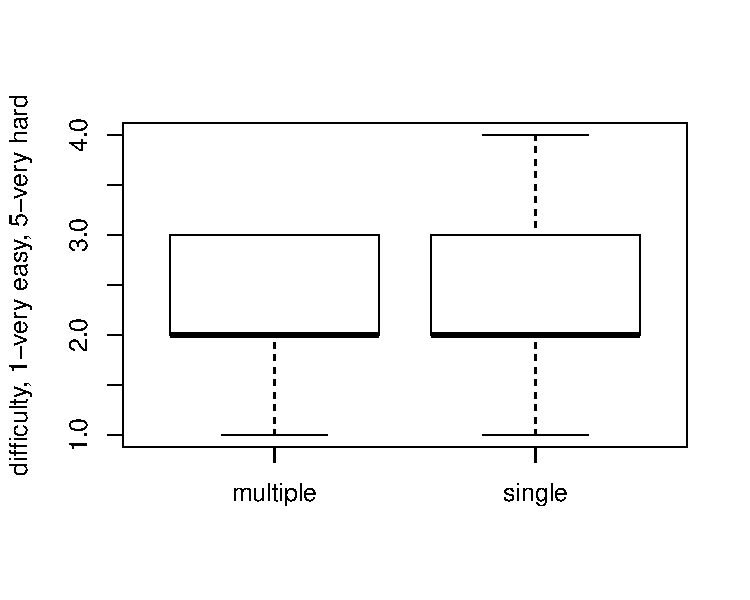
\includegraphics[width=0.5\textwidth]{figure/minimal-compare-diff-d1} 

}


\end{knitrout}


\subsection{Compare between versions: \% correct on indetifying argument and function}
1 means correct, 0 means false.

\begin{knitrout}
\definecolor{shadecolor}{rgb}{0.969, 0.969, 0.969}\color{fgcolor}\begin{kframe}
\begin{flushleft}
\ttfamily\noindent
\hlsymbol{d1}\hlkeyword{\usebox{\hlnormalsizeboxdollar}}\hlsymbol{identify\usebox{\hlnormalsizeboxunderscore}args\usebox{\hlnormalsizeboxunderscore}score}{\ }\hlassignement{\usebox{\hlnormalsizeboxlessthan}-}{\ }\hlnumber{NA}\hspace*{\fill}\\
\hlstd{}\hlsymbol{d1}\hlkeyword{\usebox{\hlnormalsizeboxdollar}}\hlsymbol{identify\usebox{\hlnormalsizeboxunderscore}args\usebox{\hlnormalsizeboxunderscore}score}\hlkeyword{[}\hlsymbol{d1}\hlkeyword{\usebox{\hlnormalsizeboxdollar}}\hlsymbol{identify\usebox{\hlnormalsizeboxunderscore}args}{\ }=={\ }\hlstring{"{}function:{\ }names,{\ }argument:{\ }present"{}}\hlkeyword{]}{\ }\hlassignement{\usebox{\hlnormalsizeboxlessthan}-}{\ }\hlnumber{1}\hspace*{\fill}\\
\hlstd{}\hlsymbol{d1}\hlkeyword{\usebox{\hlnormalsizeboxdollar}}\hlsymbol{identify\usebox{\hlnormalsizeboxunderscore}args\usebox{\hlnormalsizeboxunderscore}score}\hlkeyword{[}\hlsymbol{d1}\hlkeyword{\usebox{\hlnormalsizeboxdollar}}\hlsymbol{identify\usebox{\hlnormalsizeboxunderscore}args}{\ }=={\ }\hlstring{"{}function:{\ }present,{\ }argument:{\ }names"{}}\hlkeyword{]}{\ }\hlassignement{\usebox{\hlnormalsizeboxlessthan}-}{\ }\hlnumber{0}\hspace*{\fill}\\
\hlstd{}\hlfunctioncall{mosaicplot}\hlkeyword{(}\hlfunctioncall{table}\hlkeyword{(}\hlsymbol{d1}\hlkeyword{\usebox{\hlnormalsizeboxdollar}}\hlsymbol{color}\hlkeyword{,}{\ }\hlsymbol{d1}\hlkeyword{\usebox{\hlnormalsizeboxdollar}}\hlsymbol{identify\usebox{\hlnormalsizeboxunderscore}args\usebox{\hlnormalsizeboxunderscore}score}\hlkeyword{)}\hlkeyword{)}\hspace*{\fill}\\
\hlstd{}\hlfunctioncall{chisq.test}\hlkeyword{(}\hlfunctioncall{table}\hlkeyword{(}\hlsymbol{d1}\hlkeyword{\usebox{\hlnormalsizeboxdollar}}\hlsymbol{color}\hlkeyword{,}{\ }\hlsymbol{d1}\hlkeyword{\usebox{\hlnormalsizeboxdollar}}\hlsymbol{identify\usebox{\hlnormalsizeboxunderscore}args\usebox{\hlnormalsizeboxunderscore}score}\hlkeyword{)}\hlkeyword{,}{\ }\hlargument{simulate.p.value}{\ }\hlargument{=}{\ }\hlnumber{TRUE}\hlkeyword{)}\mbox{}
\normalfont
\end{flushleft}
\begin{verbatim}
## 
## 	Pearson's Chi-squared test with simulated p-value (based on 2000 replicates)
## 
## data:  table(d1$color, d1$identify_args_score) 
## X-squared = 2.123, df = NA, p-value = 0.2089
## 
\end{verbatim}
\end{kframe}

{\centering 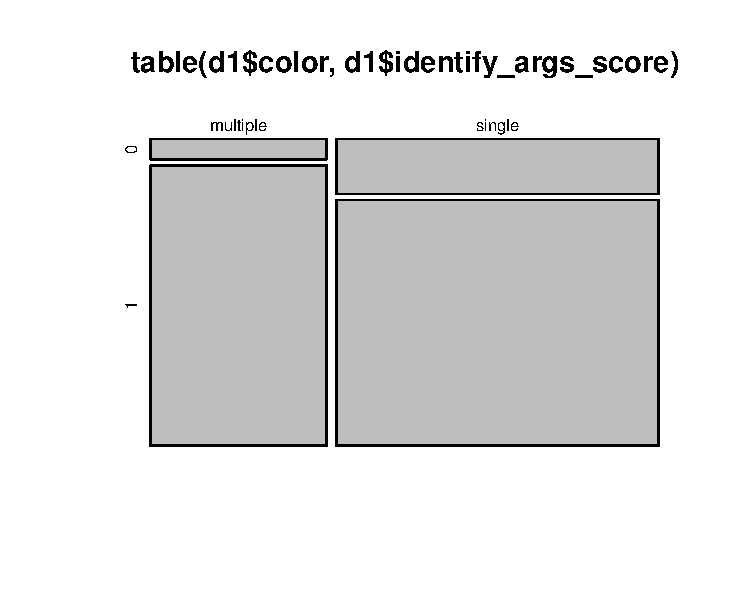
\includegraphics[width=0.5\textwidth]{figure/minimal-compare-identify_args-d1} 

}


\end{knitrout}


\subsection{Compare between versions: \%correct on number of argument}

\begin{knitrout}
\definecolor{shadecolor}{rgb}{0.969, 0.969, 0.969}\color{fgcolor}\begin{kframe}
\begin{flushleft}
\ttfamily\noindent
\hlsymbol{d1}\hlkeyword{\usebox{\hlnormalsizeboxdollar}}\hlsymbol{no\usebox{\hlnormalsizeboxunderscore}args\usebox{\hlnormalsizeboxunderscore}score}{\ }\hlassignement{\usebox{\hlnormalsizeboxlessthan}-}{\ }\hlnumber{NA}\hspace*{\fill}\\
\hlstd{}\hlsymbol{d1}\hlkeyword{\usebox{\hlnormalsizeboxdollar}}\hlsymbol{no\usebox{\hlnormalsizeboxunderscore}args\usebox{\hlnormalsizeboxunderscore}score}\hlkeyword{[}\hlsymbol{d1}\hlkeyword{\usebox{\hlnormalsizeboxdollar}}\hlsymbol{no\usebox{\hlnormalsizeboxunderscore}args}{\ }=={\ }\hlnumber{3}\hlkeyword{]}{\ }\hlassignement{\usebox{\hlnormalsizeboxlessthan}-}{\ }\hlnumber{1}\hspace*{\fill}\\
\hlstd{}\hlsymbol{d1}\hlkeyword{\usebox{\hlnormalsizeboxdollar}}\hlsymbol{no\usebox{\hlnormalsizeboxunderscore}args\usebox{\hlnormalsizeboxunderscore}score}\hlkeyword{[}\hlsymbol{d1}\hlkeyword{\usebox{\hlnormalsizeboxdollar}}\hlsymbol{no\usebox{\hlnormalsizeboxunderscore}args}{\ }\hlkeyword{!=}{\ }\hlnumber{3}\hlkeyword{]}{\ }\hlassignement{\usebox{\hlnormalsizeboxlessthan}-}{\ }\hlnumber{0}\hspace*{\fill}\\
\hlstd{}\hlfunctioncall{mosaicplot}\hlkeyword{(}\hlfunctioncall{table}\hlkeyword{(}\hlsymbol{d1}\hlkeyword{\usebox{\hlnormalsizeboxdollar}}\hlsymbol{color}\hlkeyword{,}{\ }\hlsymbol{d1}\hlkeyword{\usebox{\hlnormalsizeboxdollar}}\hlsymbol{no\usebox{\hlnormalsizeboxunderscore}args\usebox{\hlnormalsizeboxunderscore}score}\hlkeyword{)}\hlkeyword{)}\hspace*{\fill}\\
\hlstd{}\hlfunctioncall{chisq.test}\hlkeyword{(}\hlfunctioncall{table}\hlkeyword{(}\hlsymbol{d1}\hlkeyword{\usebox{\hlnormalsizeboxdollar}}\hlsymbol{color}\hlkeyword{,}{\ }\hlsymbol{d1}\hlkeyword{\usebox{\hlnormalsizeboxdollar}}\hlsymbol{no\usebox{\hlnormalsizeboxunderscore}args\usebox{\hlnormalsizeboxunderscore}score}\hlkeyword{)}\hlkeyword{)}\mbox{}
\normalfont
\end{flushleft}
\begin{verbatim}
## 
## 	Pearson's Chi-squared test with Yates' continuity correction
## 
## data:  table(d1$color, d1$no_args_score) 
## X-squared = 0.0016, df = 1, p-value = 0.9679
## 
\end{verbatim}
\end{kframe}

{\centering 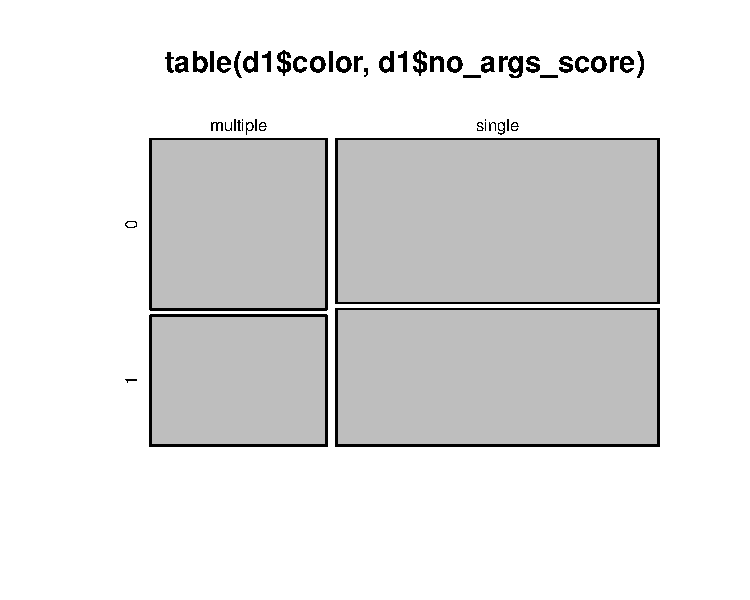
\includegraphics[width=0.5\textwidth]{figure/minimal-compare-no_args-d1} 

}


\end{knitrout}


\section{Week 2}

Survey can be found at: \\
\href{https://docs.google.com/spreadsheet/viewform?formkey=dHlCMFl2ZmtHT2lDdXR4U0VKWmlicnc6MQ#gid=0}{https://docs.google.com/spreadsheet/viewform?formkey=dHlCMFl2ZmtHT2lDdXR4U0VKWmlicnc6MQ\#gid=0}

\begin{knitrout}
\definecolor{shadecolor}{rgb}{0.969, 0.969, 0.969}\color{fgcolor}\begin{kframe}
\begin{flushleft}
\ttfamily\noindent
\hlsymbol{d2}{\ }\hlassignement{=}{\ }\hlfunctioncall{read.csv}\hlkeyword{(}\hlstring{"{}Lab{\ }survey{\ }-{\ }Week{\ }2{\ }-{\ }Sheet1.csv"{}}\hlkeyword{)}\hspace*{\fill}\\
\hlstd{}\hlfunctioncall{names}\hlkeyword{(}\hlsymbol{d2}\hlkeyword{)}{\ }\hlassignement{=}{\ }\hlfunctioncall{c}\hlkeyword{(}\hlstring{"{}timestamp"{}}\hlkeyword{,}\hlstring{"{}difficulty"{}}\hlkeyword{,}\hlstring{"{}whats\usebox{\hlnormalsizeboxunderscore}wrong1"{}}\hlkeyword{,}\hlstring{"{}whats\usebox{\hlnormalsizeboxunderscore}wrong2"{}}\hlkeyword{,}\hlstring{"{}compare\usebox{\hlnormalsizeboxunderscore}diff"{}}\hlkeyword{,}\hspace*{\fill}\\
\hlstd{}{\ }{\ }{\ }{\ }{\ }{\ }{\ }{\ }{\ }{\ }{\ }{\ }{\ }{\ }\hlstring{"{}rewrite"{}}\hlkeyword{,}{\ }\hlstring{"{}rewrite\usebox{\hlnormalsizeboxunderscore}score"{}}\hlkeyword{,}\hlstring{"{}typos"{}}\hlkeyword{,}\hlstring{"{}color"{}}\hlkeyword{,}\hlstring{"{}identifier"{}}\hlkeyword{)}\hspace*{\fill}\\
\hlstd{}\hlfunctioncall{levels}\hlkeyword{(}\hlsymbol{d2}\hlkeyword{\usebox{\hlnormalsizeboxdollar}}\hlsymbol{color}\hlkeyword{)}{\ }\hlassignement{=}{\ }\hlfunctioncall{c}\hlkeyword{(}\hlstring{"{}multiple"{}}\hlkeyword{,}\hlstring{"{}single"{}}\hlkeyword{)}\hspace*{\fill}\\
\hlstd{}\hlfunctioncall{dim}\hlkeyword{(}\hlsymbol{d2}\hlkeyword{)}\mbox{}
\normalfont
\end{flushleft}
\begin{verbatim}
## [1] 77 10
\end{verbatim}
\end{kframe}
\end{knitrout}


I assigned scores to the open-ended rewrite the code question manually. There was no partial credit, so those that had only a minor mistake (spell \hlsymbol{mosaicplot} as \hlsymbol{Mosaicplot}) received the same score as a major mistake or no answer.

\subsection{Compare between versions: difficulty}

\begin{knitrout}
\definecolor{shadecolor}{rgb}{0.969, 0.969, 0.969}\color{fgcolor}\begin{kframe}
\begin{flushleft}
\ttfamily\noindent
\hlfunctioncall{boxplot}\hlkeyword{(}\hlsymbol{d2}\hlkeyword{\usebox{\hlnormalsizeboxdollar}}\hlsymbol{difficulty}{\ }\hlkeyword{\urltilda{}}{\ }\hlsymbol{d2}\hlkeyword{\usebox{\hlnormalsizeboxdollar}}\hlsymbol{color}\hlkeyword{,}{\ }\hlargument{ylab}{\ }\hlargument{=}{\ }\hlstring{"{}difficulty,{\ }1-very{\ }easy,{\ }5-very{\ }hard"{}}\hlkeyword{)}\hspace*{\fill}\\
\hlstd{}\hlfunctioncall{t.test}\hlkeyword{(}\hlsymbol{d2}\hlkeyword{\usebox{\hlnormalsizeboxdollar}}\hlsymbol{difficulty}{\ }\hlkeyword{\urltilda{}}{\ }\hlsymbol{d2}\hlkeyword{\usebox{\hlnormalsizeboxdollar}}\hlsymbol{color}\hlkeyword{)}\mbox{}
\normalfont
\end{flushleft}
\begin{verbatim}
## 
## 	Welch Two Sample t-test
## 
## data:  d2$difficulty by d2$color 
## t = -1.911, df = 74.27, p-value = 0.05981
## alternative hypothesis: true difference in means is not equal to 0 
## 95 percent confidence interval:
##  -0.65323  0.01355 
## sample estimates:
## mean in group multiple   mean in group single 
##                  3.154                  3.474 
## 
\end{verbatim}
\end{kframe}

{\centering 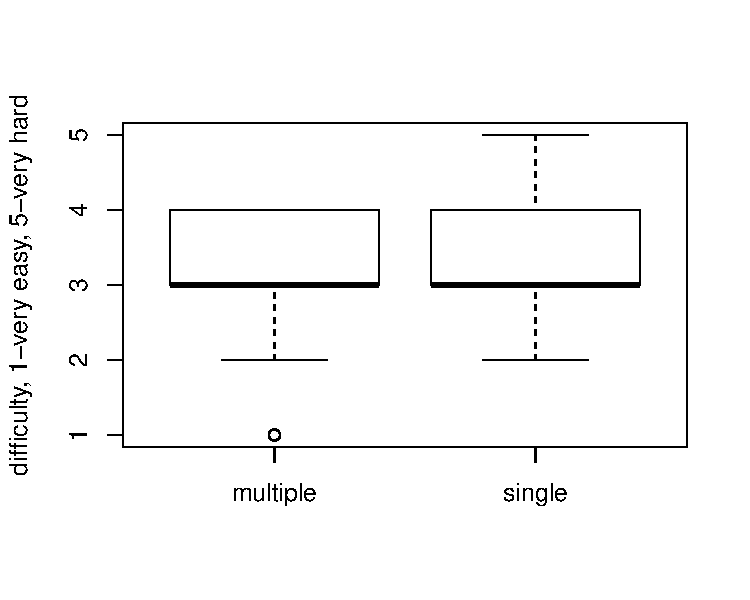
\includegraphics[width=0.5\textwidth]{figure/minimal-compare-diff-d2} 

}


\end{knitrout}


\subsection{Compare between versions: what's wrong with the code (1)}

\begin{knitrout}
\definecolor{shadecolor}{rgb}{0.969, 0.969, 0.969}\color{fgcolor}\begin{kframe}
\begin{flushleft}
\ttfamily\noindent
\hlsymbol{d2}\hlkeyword{\usebox{\hlnormalsizeboxdollar}}\hlsymbol{whats\usebox{\hlnormalsizeboxunderscore}wrong1\usebox{\hlnormalsizeboxunderscore}score}{\ }\hlassignement{\usebox{\hlnormalsizeboxlessthan}-}{\ }\hlnumber{NA}\hspace*{\fill}\\
\hlstd{}\hlsymbol{d2}\hlkeyword{\usebox{\hlnormalsizeboxdollar}}\hlsymbol{whats\usebox{\hlnormalsizeboxunderscore}wrong1\usebox{\hlnormalsizeboxunderscore}score}\hlkeyword{[}\hlsymbol{d2}\hlkeyword{\usebox{\hlnormalsizeboxdollar}}\hlsymbol{whats\usebox{\hlnormalsizeboxunderscore}wrong1}{\ }=={\ }\hlstring{"{}30{\ }should{\ }not{\ }be{\ }in{\ }quotation{\ }marks."{}}\hlkeyword{]}{\ }\hlassignement{\usebox{\hlnormalsizeboxlessthan}-}{\ }\hlnumber{1}\hspace*{\fill}\\
\hlstd{}\hlsymbol{d2}\hlkeyword{\usebox{\hlnormalsizeboxdollar}}\hlsymbol{whats\usebox{\hlnormalsizeboxunderscore}wrong1\usebox{\hlnormalsizeboxunderscore}score}\hlkeyword{[}\hlsymbol{d2}\hlkeyword{\usebox{\hlnormalsizeboxdollar}}\hlsymbol{whats\usebox{\hlnormalsizeboxunderscore}wrong1}{\ }\hlkeyword{!=}{\ }\hlstring{"{}30{\ }should{\ }not{\ }be{\ }in{\ }quotation{\ }marks."{}}\hlkeyword{]}{\ }\hlassignement{\usebox{\hlnormalsizeboxlessthan}-}{\ }\hlnumber{0}\hspace*{\fill}\\
\hlstd{}\hlfunctioncall{mosaicplot}\hlkeyword{(}\hlfunctioncall{table}\hlkeyword{(}\hlsymbol{d2}\hlkeyword{\usebox{\hlnormalsizeboxdollar}}\hlsymbol{color}\hlkeyword{,}{\ }\hlsymbol{d2}\hlkeyword{\usebox{\hlnormalsizeboxdollar}}\hlsymbol{whats\usebox{\hlnormalsizeboxunderscore}wrong1\usebox{\hlnormalsizeboxunderscore}score}\hlkeyword{)}\hlkeyword{)}\hspace*{\fill}\\
\hlstd{}\hlfunctioncall{chisq.test}\hlkeyword{(}\hlfunctioncall{table}\hlkeyword{(}\hlsymbol{d2}\hlkeyword{\usebox{\hlnormalsizeboxdollar}}\hlsymbol{color}\hlkeyword{,}{\ }\hlsymbol{d2}\hlkeyword{\usebox{\hlnormalsizeboxdollar}}\hlsymbol{whats\usebox{\hlnormalsizeboxunderscore}wrong1\usebox{\hlnormalsizeboxunderscore}score}\hlkeyword{)}\hlkeyword{)}\mbox{}
\normalfont
\end{flushleft}
\begin{verbatim}
## 
## 	Pearson's Chi-squared test with Yates' continuity correction
## 
## data:  table(d2$color, d2$whats_wrong1_score) 
## X-squared = 1.821, df = 1, p-value = 0.1772
## 
\end{verbatim}
\end{kframe}

{\centering 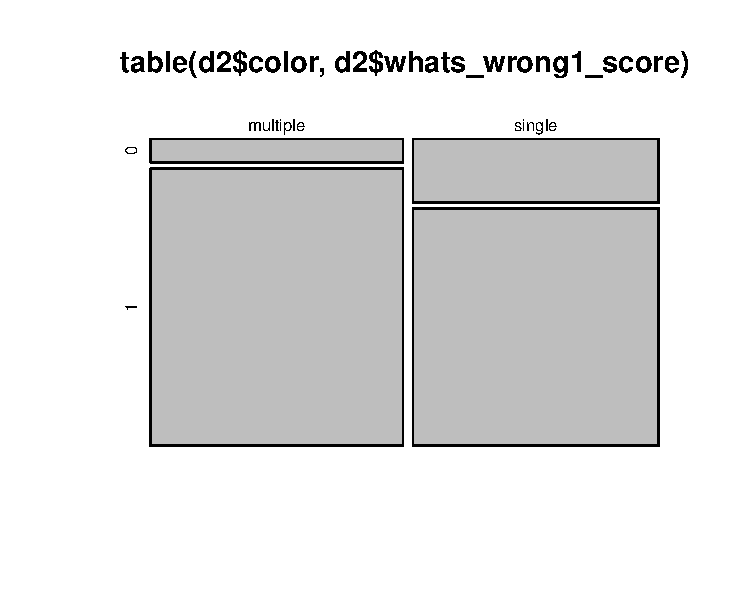
\includegraphics[width=0.5\textwidth]{figure/minimal-compare-whats_wrong1-d2} 

}


\end{knitrout}


\subsection{Compare between versions: what's wrong with the code (2)}

\begin{knitrout}
\definecolor{shadecolor}{rgb}{0.969, 0.969, 0.969}\color{fgcolor}\begin{kframe}
\begin{flushleft}
\ttfamily\noindent
\hlsymbol{d2}\hlkeyword{\usebox{\hlnormalsizeboxdollar}}\hlsymbol{whats\usebox{\hlnormalsizeboxunderscore}wrong2\usebox{\hlnormalsizeboxunderscore}score}{\ }\hlassignement{\usebox{\hlnormalsizeboxlessthan}-}{\ }\hlnumber{NA}\hspace*{\fill}\\
\hlstd{}\hlsymbol{d2}\hlkeyword{\usebox{\hlnormalsizeboxdollar}}\hlsymbol{whats\usebox{\hlnormalsizeboxunderscore}wrong2\usebox{\hlnormalsizeboxunderscore}score}\hlkeyword{[}\hlsymbol{d2}\hlkeyword{\usebox{\hlnormalsizeboxdollar}}\hlsymbol{whats\usebox{\hlnormalsizeboxunderscore}wrong2}{\ }=={\ }\hlstring{"{}{\ }={\ }should{\ }instead{\ }be{\ }==."{}}\hlkeyword{]}{\ }\hlassignement{\usebox{\hlnormalsizeboxlessthan}-}{\ }\hlnumber{1}\hspace*{\fill}\\
\hlstd{}\hlsymbol{d2}\hlkeyword{\usebox{\hlnormalsizeboxdollar}}\hlsymbol{whats\usebox{\hlnormalsizeboxunderscore}wrong2\usebox{\hlnormalsizeboxunderscore}score}\hlkeyword{[}\hlsymbol{d2}\hlkeyword{\usebox{\hlnormalsizeboxdollar}}\hlsymbol{whats\usebox{\hlnormalsizeboxunderscore}wrong2}{\ }\hlkeyword{!=}{\ }\hlstring{"{}{\ }={\ }should{\ }instead{\ }be{\ }==."{}}\hlkeyword{]}{\ }\hlassignement{\usebox{\hlnormalsizeboxlessthan}-}{\ }\hlnumber{0}\hspace*{\fill}\\
\hlstd{}\hlfunctioncall{mosaicplot}\hlkeyword{(}\hlfunctioncall{table}\hlkeyword{(}\hlsymbol{d2}\hlkeyword{\usebox{\hlnormalsizeboxdollar}}\hlsymbol{color}\hlkeyword{,}{\ }\hlsymbol{d2}\hlkeyword{\usebox{\hlnormalsizeboxdollar}}\hlsymbol{whats\usebox{\hlnormalsizeboxunderscore}wrong2\usebox{\hlnormalsizeboxunderscore}score}\hlkeyword{)}\hlkeyword{)}\hspace*{\fill}\\
\hlstd{}\hlfunctioncall{chisq.test}\hlkeyword{(}\hlfunctioncall{table}\hlkeyword{(}\hlsymbol{d2}\hlkeyword{\usebox{\hlnormalsizeboxdollar}}\hlsymbol{color}\hlkeyword{,}{\ }\hlsymbol{d2}\hlkeyword{\usebox{\hlnormalsizeboxdollar}}\hlsymbol{whats\usebox{\hlnormalsizeboxunderscore}wrong2\usebox{\hlnormalsizeboxunderscore}score}\hlkeyword{)}\hlkeyword{,}{\ }\hlargument{simulate.p.value}{\ }\hlargument{=}{\ }\hlnumber{TRUE}\hlkeyword{)}\mbox{}
\normalfont
\end{flushleft}
\begin{verbatim}
## 
## 	Pearson's Chi-squared test with simulated p-value (based on 2000 replicates)
## 
## data:  table(d2$color, d2$whats_wrong2_score) 
## X-squared = 0.0011, df = NA, p-value = 1
## 
\end{verbatim}
\end{kframe}

{\centering 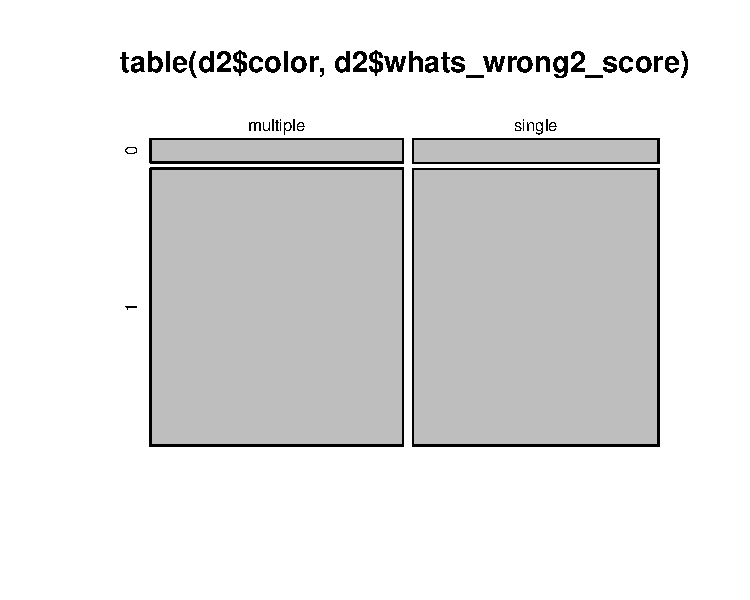
\includegraphics[width=0.5\textwidth]{figure/minimal-compare-whats_wrong2-d2} 

}


\end{knitrout}


\subsection{Compare between versions: \%correct on rewrite}

\begin{knitrout}
\definecolor{shadecolor}{rgb}{0.969, 0.969, 0.969}\color{fgcolor}\begin{kframe}
\begin{flushleft}
\ttfamily\noindent
\hlfunctioncall{mosaicplot}\hlkeyword{(}\hlfunctioncall{table}\hlkeyword{(}\hlsymbol{d2}\hlkeyword{\usebox{\hlnormalsizeboxdollar}}\hlsymbol{color}\hlkeyword{,}{\ }\hlsymbol{d2}\hlkeyword{\usebox{\hlnormalsizeboxdollar}}\hlsymbol{rewrite\usebox{\hlnormalsizeboxunderscore}score}\hlkeyword{)}\hlkeyword{)}\hspace*{\fill}\\
\hlstd{}\hlfunctioncall{chisq.test}\hlkeyword{(}\hlfunctioncall{table}\hlkeyword{(}\hlsymbol{d2}\hlkeyword{\usebox{\hlnormalsizeboxdollar}}\hlsymbol{color}\hlkeyword{,}{\ }\hlsymbol{d2}\hlkeyword{\usebox{\hlnormalsizeboxdollar}}\hlsymbol{rewrite\usebox{\hlnormalsizeboxunderscore}score}\hlkeyword{)}\hlkeyword{)}\mbox{}
\normalfont
\end{flushleft}
\begin{verbatim}
## 
## 	Pearson's Chi-squared test with Yates' continuity correction
## 
## data:  table(d2$color, d2$rewrite_score) 
## X-squared = 0.3346, df = 1, p-value = 0.5629
## 
\end{verbatim}
\end{kframe}

{\centering 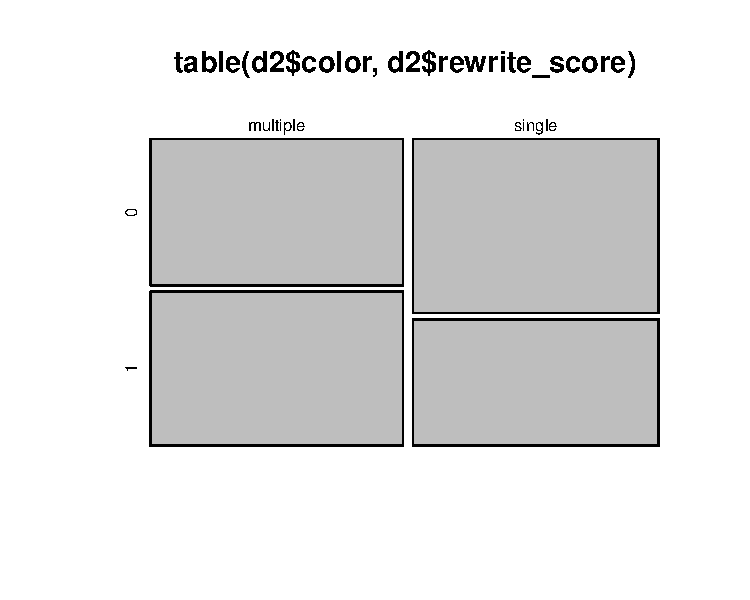
\includegraphics[width=0.5\textwidth]{figure/minimal-compare-rewrite-d2} 

}


\end{knitrout}


\subsection{Compare between versions: typos}

\begin{knitrout}
\definecolor{shadecolor}{rgb}{0.969, 0.969, 0.969}\color{fgcolor}\begin{kframe}
\begin{flushleft}
\ttfamily\noindent
\hlfunctioncall{mosaicplot}\hlkeyword{(}\hlfunctioncall{table}\hlkeyword{(}\hlsymbol{d2}\hlkeyword{\usebox{\hlnormalsizeboxdollar}}\hlsymbol{color}\hlkeyword{,}{\ }\hlsymbol{d2}\hlkeyword{\usebox{\hlnormalsizeboxdollar}}\hlsymbol{typos}\hlkeyword{)}\hlkeyword{,}{\ }\hlargument{las}{\ }\hlargument{=}{\ }\hlnumber{1}\hlkeyword{)}\hspace*{\fill}\\
\hlstd{}\hlfunctioncall{chisq.test}\hlkeyword{(}\hlfunctioncall{table}\hlkeyword{(}\hlsymbol{d2}\hlkeyword{\usebox{\hlnormalsizeboxdollar}}\hlsymbol{color}\hlkeyword{,}{\ }\hlsymbol{d2}\hlkeyword{\usebox{\hlnormalsizeboxdollar}}\hlsymbol{typos}\hlkeyword{)}\hlkeyword{,}{\ }\hlargument{simulate.p.value}{\ }\hlargument{=}{\ }\hlnumber{TRUE}\hlkeyword{)}\mbox{}
\normalfont
\end{flushleft}
\begin{verbatim}
## 
## 	Pearson's Chi-squared test with simulated p-value (based on 2000 replicates)
## 
## data:  table(d2$color, d2$typos) 
## X-squared = 3.314, df = NA, p-value = 0.3833
## 
\end{verbatim}
\end{kframe}

{\centering 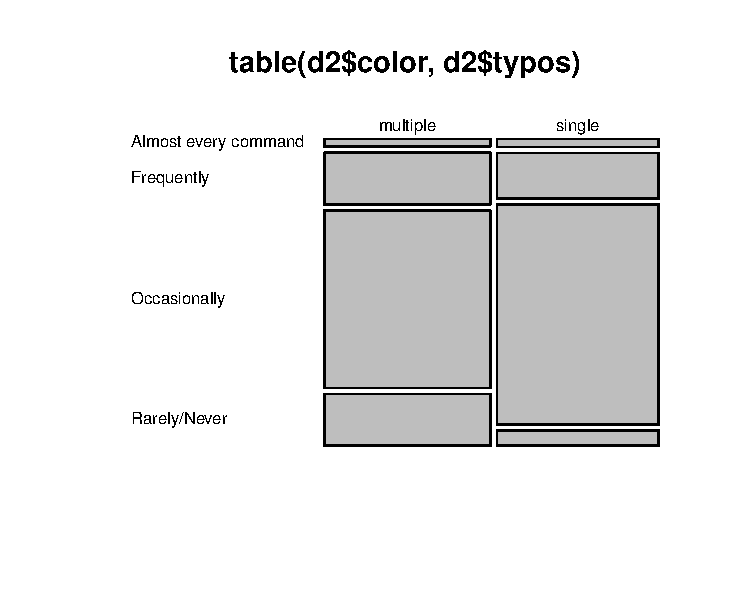
\includegraphics[width=0.5\textwidth]{figure/minimal-compare-typos-d2} 

}


\end{knitrout}


\subsection{Compare difficulty between this and previous}

\begin{knitrout}
\definecolor{shadecolor}{rgb}{0.969, 0.969, 0.969}\color{fgcolor}\begin{kframe}
\begin{flushleft}
\ttfamily\noindent
\hlfunctioncall{levels}\hlkeyword{(}\hlsymbol{d2}\hlkeyword{\usebox{\hlnormalsizeboxdollar}}\hlsymbol{compare\usebox{\hlnormalsizeboxunderscore}diff}\hlkeyword{)}{\ }\hlassignement{\usebox{\hlnormalsizeboxlessthan}-}{\ }\hlfunctioncall{c}\hlkeyword{(}\hlstring{"{}this{\ }easier"{}}\hlkeyword{,}{\ }\hlstring{"{}this{\ }more{\ }diff"{}}\hlkeyword{,}{\ }\hlstring{"{}this{\ }same"{}}\hlkeyword{)}\hspace*{\fill}\\
\hlstd{}\hlfunctioncall{mosaicplot}\hlkeyword{(}\hlfunctioncall{table}\hlkeyword{(}\hlsymbol{d2}\hlkeyword{\usebox{\hlnormalsizeboxdollar}}\hlsymbol{color}\hlkeyword{,}{\ }\hlsymbol{d2}\hlkeyword{\usebox{\hlnormalsizeboxdollar}}\hlsymbol{compare\usebox{\hlnormalsizeboxunderscore}diff}\hlkeyword{)}\hlkeyword{,}{\ }\hlargument{las}{\ }\hlargument{=}{\ }\hlnumber{1}\hlkeyword{)}\hspace*{\fill}\\
\hlstd{}\hlfunctioncall{chisq.test}\hlkeyword{(}\hlfunctioncall{table}\hlkeyword{(}\hlsymbol{d2}\hlkeyword{\usebox{\hlnormalsizeboxdollar}}\hlsymbol{color}\hlkeyword{,}{\ }\hlsymbol{d2}\hlkeyword{\usebox{\hlnormalsizeboxdollar}}\hlsymbol{compare\usebox{\hlnormalsizeboxunderscore}diff}\hlkeyword{)}\hlkeyword{,}{\ }\hlargument{simulate.p.value}{\ }\hlargument{=}{\ }\hlnumber{TRUE}\hlkeyword{)}\mbox{}
\normalfont
\end{flushleft}
\begin{verbatim}
## 
## 	Pearson's Chi-squared test with simulated p-value (based on 2000 replicates)
## 
## data:  table(d2$color, d2$compare_diff) 
## X-squared = 2.927, df = NA, p-value = 0.2894
## 
\end{verbatim}
\begin{flushleft}
\ttfamily\noindent
\hlsymbol{d2}\hlkeyword{\usebox{\hlnormalsizeboxdollar}}\hlsymbol{this\usebox{\hlnormalsizeboxunderscore}easier}{\ }\hlassignement{\usebox{\hlnormalsizeboxlessthan}-}{\ }\hlnumber{NA}\hspace*{\fill}\\
\hlstd{}\hlsymbol{d2}\hlkeyword{\usebox{\hlnormalsizeboxdollar}}\hlsymbol{this\usebox{\hlnormalsizeboxunderscore}easier}\hlkeyword{[}\hlsymbol{d2}\hlkeyword{\usebox{\hlnormalsizeboxdollar}}\hlsymbol{compare\usebox{\hlnormalsizeboxunderscore}diff}{\ }=={\ }\hlstring{"{}this{\ }easier"{}}\hlkeyword{]}{\ }\hlassignement{\usebox{\hlnormalsizeboxlessthan}-}{\ }\hlnumber{1}\hspace*{\fill}\\
\hlstd{}\hlsymbol{d2}\hlkeyword{\usebox{\hlnormalsizeboxdollar}}\hlsymbol{this\usebox{\hlnormalsizeboxunderscore}easier}\hlkeyword{[}\hlsymbol{d2}\hlkeyword{\usebox{\hlnormalsizeboxdollar}}\hlsymbol{compare\usebox{\hlnormalsizeboxunderscore}diff}{\ }\hlkeyword{!=}{\ }\hlstring{"{}this{\ }easier"{}}\hlkeyword{]}{\ }\hlassignement{\usebox{\hlnormalsizeboxlessthan}-}{\ }\hlnumber{0}\hspace*{\fill}\\
\hlstd{}\hlfunctioncall{chisq.test}\hlkeyword{(}\hlfunctioncall{table}\hlkeyword{(}\hlsymbol{d2}\hlkeyword{\usebox{\hlnormalsizeboxdollar}}\hlsymbol{color}\hlkeyword{,}{\ }\hlsymbol{d2}\hlkeyword{\usebox{\hlnormalsizeboxdollar}}\hlsymbol{this\usebox{\hlnormalsizeboxunderscore}easier}\hlkeyword{)}\hlkeyword{,}{\ }\hlargument{simulate.p.value}{\ }\hlargument{=}{\ }\hlnumber{TRUE}\hlkeyword{)}\mbox{}
\normalfont
\end{flushleft}
\begin{verbatim}
## 
## 	Pearson's Chi-squared test with simulated p-value (based on 2000 replicates)
## 
## data:  table(d2$color, d2$this_easier) 
## X-squared = 2.781, df = NA, p-value = 0.1944
## 
\end{verbatim}
\end{kframe}

{\centering 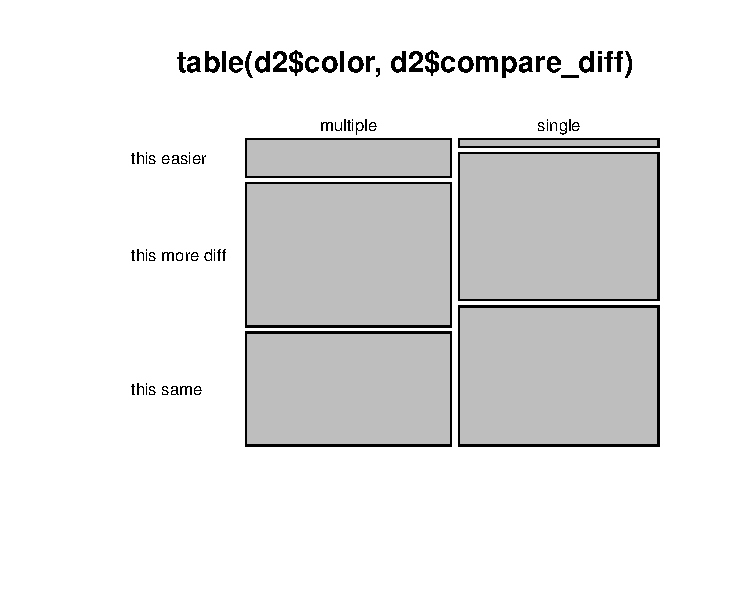
\includegraphics[width=0.5\textwidth]{figure/minimal-compare-diff-prev-d2} 

}


\end{knitrout}


\section{Compare across weeks}

Only 51 students were matched.

\begin{knitrout}
\definecolor{shadecolor}{rgb}{0.969, 0.969, 0.969}\color{fgcolor}\begin{kframe}
\begin{flushleft}
\ttfamily\noindent
\hlsymbol{d}{\ }\hlassignement{\usebox{\hlnormalsizeboxlessthan}-}{\ }\hlfunctioncall{merge}\hlkeyword{(}\hlsymbol{d1}\hlkeyword{,}{\ }\hlsymbol{d2}\hlkeyword{,}{\ }\hlargument{by}{\ }\hlargument{=}{\ }\hlfunctioncall{c}\hlkeyword{(}\hlstring{"{}identifier"{}}\hlkeyword{,}{\ }\hlstring{"{}identifier"{}}\hlkeyword{)}\hlkeyword{)}\hspace*{\fill}\\
\hlstd{}\hlsymbol{d}{\ }\hlassignement{\usebox{\hlnormalsizeboxlessthan}-}{\ }\hlsymbol{d}\hlkeyword{[}\hlsymbol{d}\hlkeyword{\usebox{\hlnormalsizeboxdollar}}\hlsymbol{identifier}{\ }\hlkeyword{!=}{\ }\hlstring{"{}123"{}}\hlkeyword{,}{\ }\hlkeyword{]}{\ }{\ }\hlcomment{\usebox{\hlnormalsizeboxhash}{\ }4{\ }people{\ }chose{\ }123!}\hspace*{\fill}\\
\hlstd{}\hlfunctioncall{dim}\hlkeyword{(}\hlsymbol{d}\hlkeyword{)}\mbox{}
\normalfont
\end{flushleft}
\begin{verbatim}
## [1] 51 20
\end{verbatim}
\end{kframe}
\end{knitrout}


\subsection{Sanity check}

There should have been nobody who had multiple or single colors both weeks, but there are. I'm confident that they got the correct links, so I think they don't quite understand what the question is asking. I don't know what this means about the reliability of the rest of the results.

\begin{knitrout}
\definecolor{shadecolor}{rgb}{0.969, 0.969, 0.969}\color{fgcolor}\begin{kframe}
\begin{flushleft}
\ttfamily\noindent
\hlfunctioncall{table}\hlkeyword{(}\hlsymbol{d}\hlkeyword{\usebox{\hlnormalsizeboxdollar}}\hlsymbol{color.x}\hlkeyword{,}{\ }\hlsymbol{d}\hlkeyword{\usebox{\hlnormalsizeboxdollar}}\hlsymbol{color.y}\hlkeyword{)}\mbox{}
\normalfont
\end{flushleft}
\begin{verbatim}
##           
##            multiple single
##   multiple       11      7
##   single         17     16
\end{verbatim}
\end{kframe}
\end{knitrout}


\subsection{Change in perceived in difficulty}

\begin{knitrout}
\definecolor{shadecolor}{rgb}{0.969, 0.969, 0.969}\color{fgcolor}\begin{kframe}
\begin{flushleft}
\ttfamily\noindent
\hlsymbol{d}\hlkeyword{\usebox{\hlnormalsizeboxdollar}}\hlsymbol{diff\usebox{\hlnormalsizeboxunderscore}diff}{\ }\hlassignement{\usebox{\hlnormalsizeboxlessthan}-}{\ }\hlsymbol{d}\hlkeyword{\usebox{\hlnormalsizeboxdollar}}\hlsymbol{difficulty.x}{\ }\hlkeyword{-}{\ }\hlsymbol{d}\hlkeyword{\usebox{\hlnormalsizeboxdollar}}\hlsymbol{difficulty.y}\hspace*{\fill}\\
\hlstd{}\hlfunctioncall{boxplot}\hlkeyword{(}\hlsymbol{d}\hlkeyword{\usebox{\hlnormalsizeboxdollar}}\hlsymbol{diff\usebox{\hlnormalsizeboxunderscore}diff}{\ }\hlkeyword{\urltilda{}}{\ }\hlsymbol{d}\hlkeyword{\usebox{\hlnormalsizeboxdollar}}\hlsymbol{color.x}\hlkeyword{,}{\ }\hlargument{xlab}{\ }\hlargument{=}{\ }\hlstring{"{}color{\ }in{\ }week{\ }1"{}}\hlkeyword{,}{\ }\hlargument{ylab}{\ }\hlargument{=}{\ }\hlstring{"{}week{\ }1{\ }difficulty{\ }-{\ }week{\ }2{\ }difficulty"{}}\hlkeyword{)}\hspace*{\fill}\\
\hlstd{}\hlfunctioncall{boxplot}\hlkeyword{(}\hlsymbol{d}\hlkeyword{\usebox{\hlnormalsizeboxdollar}}\hlsymbol{diff\usebox{\hlnormalsizeboxunderscore}diff}{\ }\hlkeyword{\urltilda{}}{\ }\hlsymbol{d}\hlkeyword{\usebox{\hlnormalsizeboxdollar}}\hlsymbol{color.y}\hlkeyword{,}{\ }\hlargument{xlab}{\ }\hlargument{=}{\ }\hlstring{"{}color{\ }in{\ }week{\ }2"{}}\hlkeyword{,}{\ }\hlargument{ylab}{\ }\hlargument{=}{\ }\hlstring{"{}week{\ }1{\ }difficulty{\ }-{\ }week{\ }2{\ }difficulty"{}}\hlkeyword{)}\mbox{}
\normalfont
\end{flushleft}
\end{kframe}

{\centering 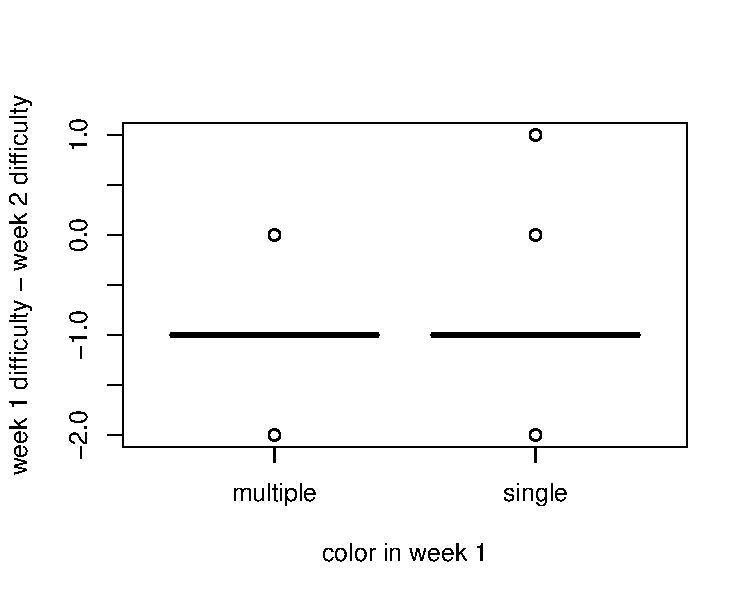
\includegraphics[width=0.5\textwidth]{figure/minimal-diff-diff1} 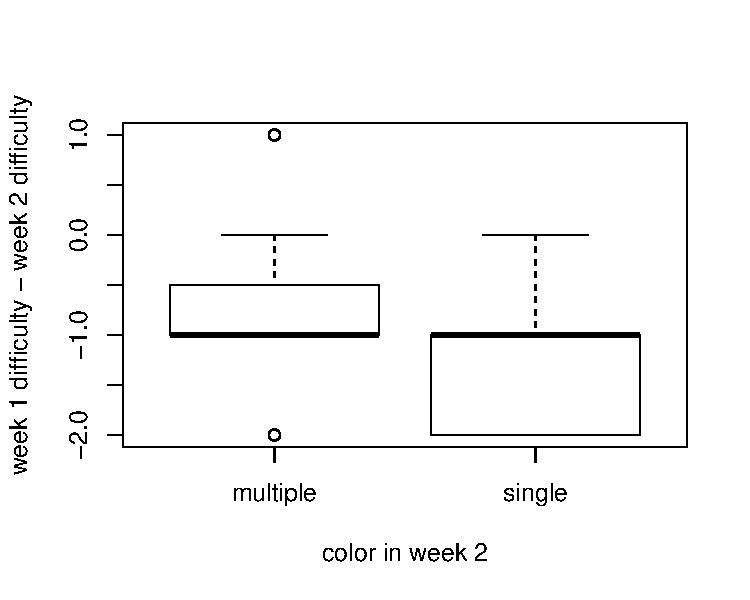
\includegraphics[width=0.5\textwidth]{figure/minimal-diff-diff2} 

}


\end{knitrout}


\end{document}
